\section{Basic Unlinkable CC Protocol}
\label{sec:unlinkable-design-1}

When the Wallet Server receives a Registration message, it stores the card information and associates a card identifier \emph{ID} with this record.
In the basic protocol, the Wallet Server responds to the Registration message with this identifier \emph{ID}.
The Wallet Application stores this value securely, associating it with the credit card being registered.
The protocol then operates as follows, and is illustrated in Figure \ref{fig:unlinkable-1}:

\begin{figure}[h!]
  \caption{Basic Unlinkable CC Protocol}
  \centering
    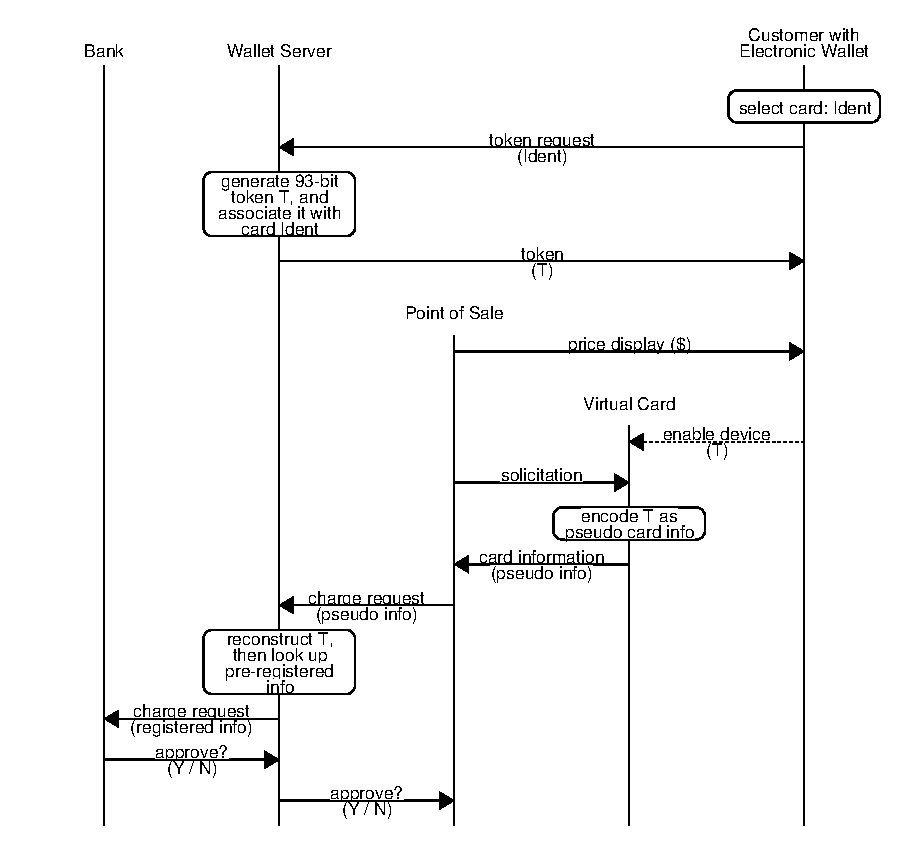
\includegraphics{img/unlinkable-1.eps}
  \label{fig:unlinkable-1}
\end{figure}

\begin{enumerate}
\item The customer selects a credit card in the Wallet Application.
\item The Wallet Application sends a Token Request message to the Wallet Server.
    This message consists of the card identifier \emph{ID} associated with the selected card, and is sent securely over the Internet.
    Note that this message must also be authenticated, to prevent a customer from requesting a token to a different customer's card.
\item The Wallet Server then generates a random 93-bit token \emph{T}, and associates it with card \emph{ID}.
    It responds to the Wallet Application with \emph{T}.
\item The Wallet Application now begins listening for Solicitation messages.
\item The point of sale sends a Solicitation message to the Wallet Application over the NFC channel.
\item The Wallet Application looks up the 93-bit token which was issued for the card selected by the customer.
    It then converts the stored token into a 28-digit number \emph{k}
    (note that 28 digits is sufficient to store a 93 bit value: $log_{10}(2^{93}) \approx 27.995$).
    Finally, it responds with an \emph{NFC} Card Information message.
    This message has the following fields:
    \begin{itemize}
    \item \textbf{Card number:} the first 16 digits of \emph{k}
    \item \textbf{Expiration date:} the subsequent 4 digits of \emph{k}
    \item \textbf{iCVV:} the remaining 8 digits of \emph{k}
    \item \textbf{Bank name:} the Wallet Server
   	\end{itemize}
\item The point of sale constructs an \emph{NFC} Charge Request message from the (pseudo) Card number, Expiration date, iCVV, and the price it wishes to charge.
    This message is sent to the bank named in the Card Information message.
    As a result, the Charge Request message is directed to the Wallet Server and \emph{not} an actual bank.
    Note that from the perspective of the point of sale, the Wallet Server appears to be a bank like any other.
\item The Wallet Server reconstructs \emph{k} from the Charge Request message, and computes the 93-bit token it represents.
    The Wallet Server then searches its database for this token, to identify the card used in this transaction.
    If no result is found, the Wallet Server sends a ``declined'' Acceptance message to the point of sale, and aborts the protocol.
    Otherwise, the stored card details are retrieved from the Wallet Server's database.
    The Wallet Server then invalidates token \emph{k}, and sends a \emph{visual} Charge Request to the card's bank with the following fields:
    \begin{itemize}
    \item Cardholder name
    \item Card number
    \item Expiration date
    \item Billing address
    \end{itemize}
    Note that unlike the Card Information message sent by the Wallet Application, this data reflects the actual credit card information.
\item The bank receives the \emph{visual} Charge Request from the Wallet Server,
    and processes this transaction as normal.
    Finally, it responds to the Wallet Server with an Acceptance message indicating whether the charge has been accepted.
\item The Wallet Server forwards the bank's Acceptance message to the point of sale.
\end{enumerate}

Note that in this protocol, the Wallet Server has a dual role:
to the point of sale, the Wallet Server appears to be a bank, while to the bank, the Wallet Server appears to be a point of sale.

Once the transaction is complete, the Wallet Application must now request a new token from the Wallet Server for that virtual credit card.
This exchange happens securely over the Internet, and must occur each time the customer wishes to make a purchase.
Should a connection to the Internet be unavailable to the Wallet Application,
    the customer is unable to perform subsequent purchases with this virtual credit card until this exchange can take place.

This protocol is unlinkable,
    because the information received by the point of sale consists solely of a random value, accompanied by a bank name identifying the Wallet Server.
Any credit card can be used in this protocol,
    because the bank receives \emph{visual} Charge Request messages, and all credit cards support the visual interface.
Finally, this protocol uses existing infrastructure,
    in that the behaviors of the point of sale and the bank are unchanged from those of the Insecure CC Protocol.
